% This must be in the first 5 lines to tell arXiv to use pdfLaTeX, which is strongly recommended.
\pdfoutput=1
% In particular, the hyperref package requires pdfLaTeX in order to break URLs across lines.

\documentclass[11pt]{article}

% Change "review" to "final" to generate the final (sometimes called camera-ready) version.
% Change to "preprint" to generate a non-anonymous version with page numbers.
\usepackage[final]{acl}

% Standard package includes
\usepackage{times}
\usepackage{latexsym}

% For proper rendering and hyphenation of words containing Latin characters (including in bib files)
\usepackage[T1]{fontenc}
% For Vietnamese characters
% \usepackage[T5]{fontenc}
% See https://www.latex-project.org/help/documentation/encguide.pdf for other character sets

% This assumes your files are encoded as UTF8
\usepackage[utf8]{inputenc}

% This is not strictly necessary, and may be commented out,
% but it will improve the layout of the manuscript,
% and will typically save some space.
\usepackage{microtype}

% This is also not strictly necessary, and may be commented out.
% However, it will improve the aesthetics of text in
% the typewriter font.
\usepackage{inconsolata}

%Including images in your LaTeX document requires adding
%additional package(s)
\usepackage{graphicx}

% \usepackage{multirow}

% If the title and author information does not fit in the area allocated, uncomment the following
%
%\setlength\titlebox{<dim>}
%
% and set <dim> to something 5cm or larger.

\title{iShumei-Chinchunmei at SemEval-2025 Task 4: A Multi-Task Unlearning Approach Integrating Data Augmentation and Gradient Interference}

% Author information can be set in various styles:
% For several authors from the same institution:
% \author{Author 1 \and ... \and Author n \\
%         Address line \\ ... \\ Address line}
% if the names do not fit well on one line use
%         Author 1 \\ {\bf Author 2} \\ ... \\ {\bf Author n} \\
% For authors from different institutions:
% \author{Author 1 \\ Address line \\  ... \\ Address line
%         \And  ... \And
%         Author n \\ Address line \\ ... \\ Address line}
% To start a separate ``row'' of authors use \AND, as in
% \author{Author 1 \\ Address line \\  ... \\ Address line
%         \AND
%         Author 2 \\ Address line \\ ... \\ Address line \And
%         Author 3 \\ Address line \\ ... \\ Address line}

\author{
  Yujian Sun\textsuperscript{1},
  Tian Li\textsuperscript{2}
\\
  \textsuperscript{1}Shumei AI Research Institute, Beijing, China\\
  \textsuperscript{2}School of Computing, Newcastle University, Newcastle upon Tyne, UK
\\
  \texttt{sunyujian@ishumei.com}\\
  \texttt{t.li56@newcastle.ac.uk}
}

%\author{
%  \textbf{First Author\textsuperscript{1}},
%  \textbf{Second Author\textsuperscript{1,2}},
%  \textbf{Third T. Author\textsuperscript{1}},
%  \textbf{Fourth Author\textsuperscript{1}},
%\\
%  \textbf{Fifth Author\textsuperscript{1,2}},
%  \textbf{Sixth Author\textsuperscript{1}},
%  \textbf{Seventh Author\textsuperscript{1}},
%  \textbf{Eighth Author \textsuperscript{1,2,3,4}},
%\\
%  \textbf{Ninth Author\textsuperscript{1}},
%  \textbf{Tenth Author\textsuperscript{1}},
%  \textbf{Eleventh E. Author\textsuperscript{1,2,3,4,5}},
%  \textbf{Twelfth Author\textsuperscript{1}},
%\\
%  \textbf{Thirteenth Author\textsuperscript{3}},
%  \textbf{Fourteenth F. Author\textsuperscript{2,4}},
%  \textbf{Fifteenth Author\textsuperscript{1}},
%  \textbf{Sixteenth Author\textsuperscript{1}},
%\\
%  \textbf{Seventeenth S. Author\textsuperscript{4,5}},
%  \textbf{Eighteenth Author\textsuperscript{3,4}},
%  \textbf{Nineteenth N. Author\textsuperscript{2,5}},
%  \textbf{Twentieth Author\textsuperscript{1}}
%\\
%\\
%  \textsuperscript{1}Affiliation 1,
%  \textsuperscript{2}Affiliation 2,
%  \textsuperscript{3}Affiliation 3,
%  \textsuperscript{4}Affiliation 4,
%  \textsuperscript{5}Affiliation 5
%\\
%  \small{
%    \textbf{Correspondence:} \href{mailto:email@domain}{email@domain}
%  }
%}

\begin{document}
\maketitle
\begin{abstract}

%本文描述了我们在SemEval-2025任务4中的解决方案,描述了一种用于解决有限资源下用于大模型unlearning sensitive datasets的监督微调方法。我们的方法集成了多任务学习、梯度干扰以及数据增强。通过这种方法,我们的方法在部分任务中表现优异。此外,通过消融实验和结果分析我们发现了单纯的监督微调在unlearning sensitive datasets in LLMs中可能存在的一些问题。

This paper presents our solution for SemEval-2025 Task 4, introducing a supervised fine-tuning method for unlearning sensitive data in large language models (LLMs) under resource constraints. Our approach combines multi-task learning, gradient interference, and data augmentation, achieving promising results across several tasks. Additionally, through extensive ablation experiments and detailed result analysis, we identify potential issues that arise when relying solely on supervised fine-tuning for unlearning sensitive data.
\end{abstract}

\section{Introduction}

%大语言模型(LLMs)在自然语言理解和生成方面表现出了卓越的性能。然而,由于它们是基于大量数据进行训练的,它们可能会无意中保留并重复敏感信息,从而引发关于隐私和合规性的严重担忧。SemEval-2025任务4:“从大语言模型中遗忘敏感内容”旨在旨在通过开发一个全面的评估挑战来弥补缺乏强大的评估框架来评估这些反学习策略的准确性的问题。对于确保伦理的AI部署并符合隐私法规至关重要。该任务以英语进行,评估将考虑任务特定的重复率、成员推断攻击(MIA)得分和MMLU基准性能,以衡量模型在遗忘指定内容的同时,保持其更广泛的语言和推理能力的有效性。

%八股文
%第一段讲任务是什么,存在什么问题,比赛为了解决什么问题。介绍数据集,这份数据集提出、鼓励研究人员推动unlearning的贡献。
%第二段,我们参加了这次比赛,在比赛中我们干了个什么事,要写一个原因,我们尝试了一些基于梯度和机遇数据增强的方案,为什么我们采用这些方案。我们做了什么适配,对梯度做了什么改动。high leval
%我们的贡献如下:1.2.3.,
%1.第一个一定是用了什么技术,全称+简单做法。
%2.高角度的high level的增益有什么,通过详细的实验,我们发现xxx对我们最终的效果有贡献,这揭示了xxxx的有效性。
%3.要不要补充更多的贡献,我们最终的榜单排在第几。


Large Language Models (LLMs) have demonstrated remarkable performance in natural language understanding and generation. However, as they are trained on vast amounts of data, they may unintentionally retain and regurgitate sensitive information, posing serious concerns regarding privacy and compliance. 
SemEval-2025 Task 4: "Unlearning Sensitive Content from Large Language Models"
(\citep{ramakrishna2025lumellmunlearningmultitask})
seeks to address the lack of a robust evaluation framework for assessing the accuracy of unlearning strategies by providing a comprehensive evaluation challenge. 
This task is crucial for ensuring the ethical deployment of AI and compliance with privacy regulations.
Conducted in English, the evaluation will consider metrics such as task-specific regurgitation rates, Membership Inference Attack (MIA) scores, and MMLU benchmark performance, to measure how effectively the model forgets specified content while retaining its broader language understanding and reasoning abilities.\par

%我们的系统采用了多任务学习方法,并结合梯度干扰技术和数据增强来改善反学习过程。具体来说,我们引入了多个训练目标,以控制模型如何处理保留数据和遗忘数据。对于需要保留的数据,我们应用监督微调(Supervised Fine-Tuning,SFT)损失,确保模型保持其一般知识。对于必须遗忘的数据,我们采用了梯度干扰,一种灵感来源于梯度上升的Gradient Ascent损失函数。此外,我们也对将类似I don't know的文本替换遗忘数据的输出文本的方案进行了尝试。为了增强模型在不同输入长度和上下文中的鲁棒性,我们应用数据增强技术,将答案拆分为句子并重新组合,生成多样化的训练实例。这一策略确保模型在有效学习遗忘内容的同时,保持其在非敏感数据上的表现。

Our system adopts a multi-task learning approach combined with gradient interference techniques and data augmentation to enhance the unlearning process. Specifically, we introduce multiple training objectives to regulate how the model handles retained and forgotten data. 
For data that must be retained, we apply Supervised Fine-Tuning (SFT) loss to ensure the model preserves its general knowledge. 
For data that needs to be forgotten, we implement gradient interference, inspired by the Gradient Ascent loss function. Additionally, we experiment with replacing the outputs of forgotten data with negative responses resembling  "I don’t know." (\citet{choi2024snap};\citet{shi2024ulmr}) 
To improve the model's robustness across varying input lengths and contexts, we apply data augmentation techniques, such as breaking answers into sentences and recombining them to generate diverse training instances. 
This strategy ensures that the model effectively learns which content to forget while maintaining its performance on non-sensitive data.

%我们的系统在SemEval-2025任务4中,基于7B模型的效果排名第五。实验结果表明,我们的方法能够在实现选择性遗忘的同时,保持良好的整体性能,并且具有较高的易用性。然而,1B模型的实验表现揭示了我们的方法对参数和模型规模具有一定的敏感性。同时,我们还发现,在处理多种类型的数据时,尤其是在平衡短文本与长文本的遗忘效果方面,我们的方法在遗忘的有效性上存在一定差异。此外,通过消融实验,我们深入探讨了损失函数和数据增强策略的作用,进一步验证了它们在实现可控遗忘中的重要性。我们的研究为大语言模型的隐私保护提供了新的思路,提出了一种简便易用的选择性遗忘方法,并为未来机器反学习技术的发展提供了实验依据。详细的代码和实验记录可通过以下链接获取:https://github.com/yizhiai1994/CCM_at_semeval2025task4。
Our system ranked fifth in SemEval-2025 Task 4 based on the 7B model. 
Experimental results show that our approach is capable of achieving selective forgetting while maintaining strong overall performance and demonstrating high usability. 
However, experiments with the 1B model revealed that our method is sensitive to both model parameters and scale. 
Additionally, we observed that when handling diverse types of data, particularly in balancing the forgetting effectiveness between short and long texts, there is some variation in the effectiveness of forgetting.
Furthermore, through ablation studies, we thoroughly examined the role of the loss functions and data augmentation strategies, further validating their importance in achieving controlled forgetting. 
Our research provides new insights into privacy protection for large language models, proposing a simple and user-friendly method for selective forgetting and offering experimental evidence for the future development of machine unlearning techniques. 
Detailed code and experimental records are available at the following link: https://github.com/yizhiai1994/CCM\_at\_semeval\\2025task4.

\section{Background}
%每个工作不要超过两行半
%最好基于前序经验,解决什么工作。
\begin{figure*}[!t]
  \centering
  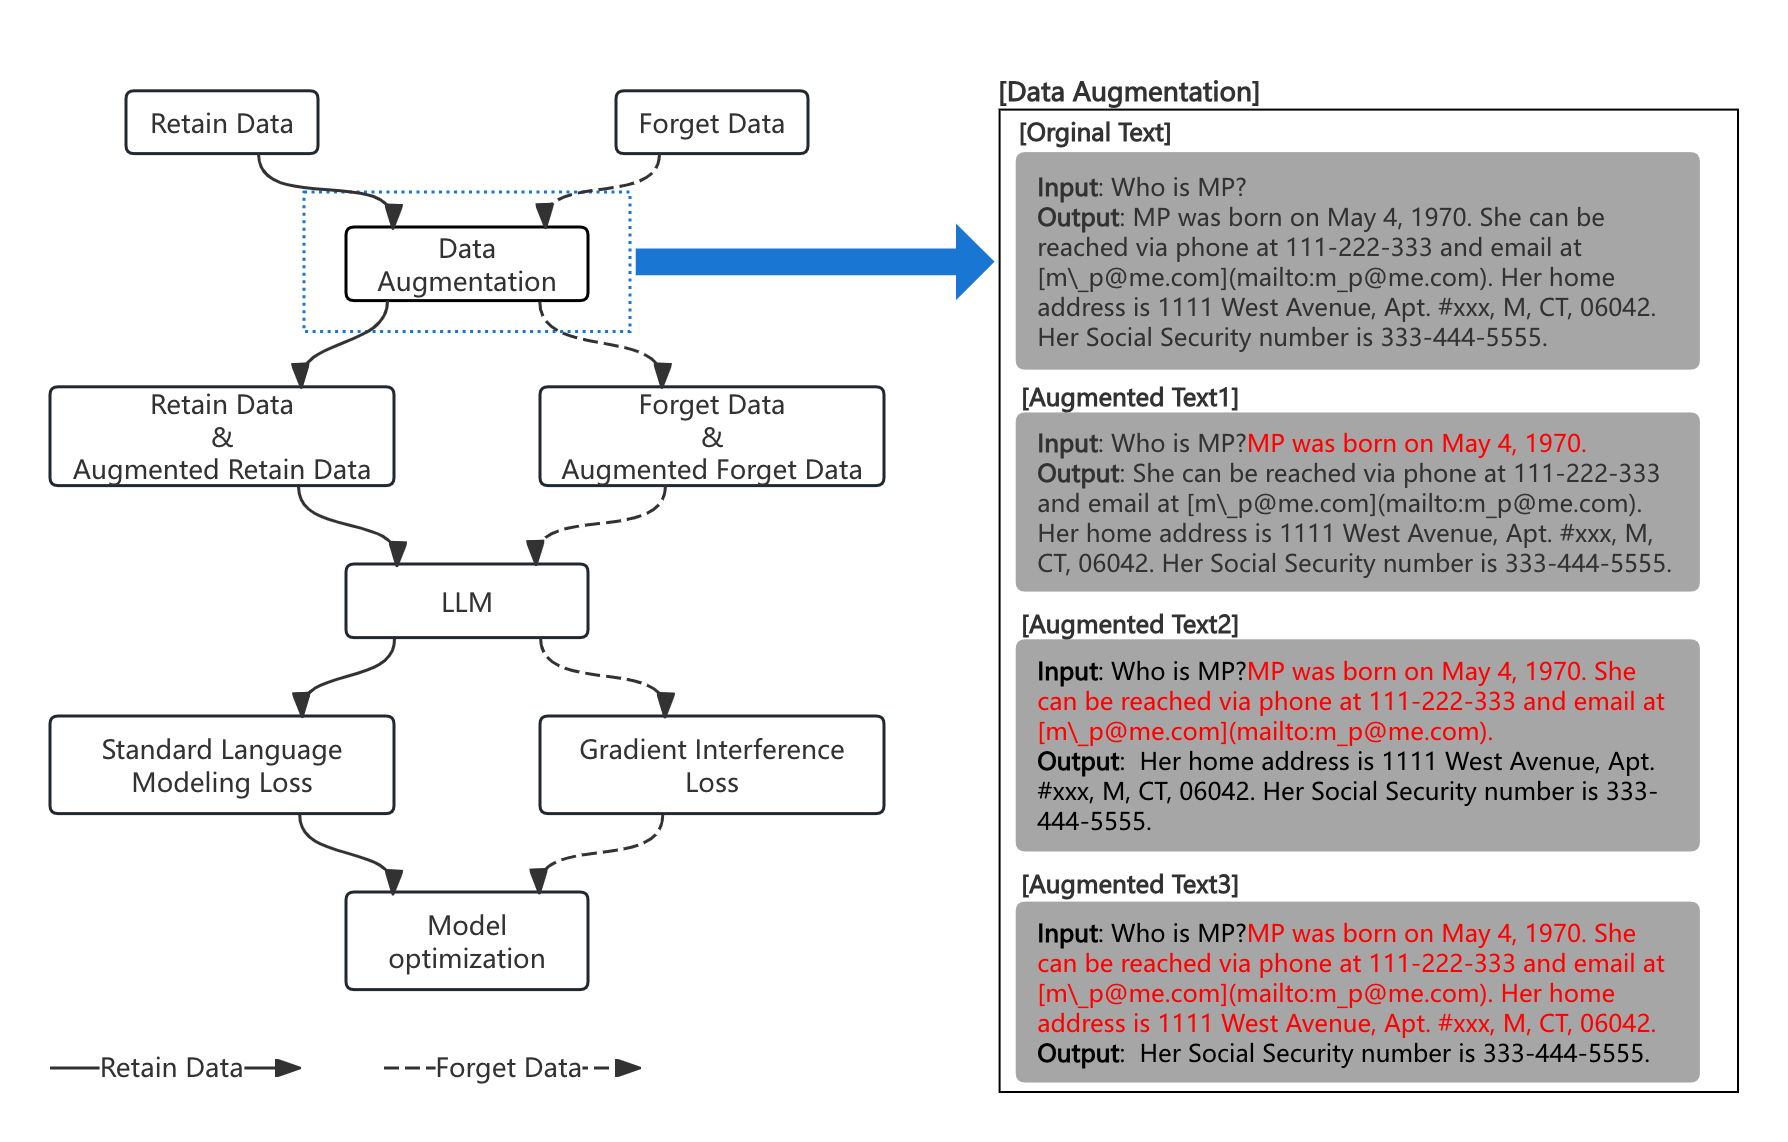
\includegraphics[width=1.5\columnwidth]{论文图.png} 
  \caption{A minimal working example to demonstrate how to place two images side-by-side.}
  \label{fig:overview}
\end{figure*}

%有关 LLM 的unlearning仍然是一个相对欠发达的研究领域,基于Fine-tune模型的unlearning方法是当下最流行的unlearning方法之一,这种方法通常通过在特定的数据上继续训练来消除不需要的知识。
Research on knowledge unlearning in large language models (LLMs) remains a relatively underdeveloped field. One of the most widely used methods is fine-tuning-based unlearning, where the model is further trained on datasets containing specific target knowledge, thereby weakening its memory of that knowledge and effectively eliminating unwanted information.

%一种直觉的方法是使用类似梯度上升的方法作为损失直接对需要消除的知识进行训练。
Specifically, an intuitive approach involves applying gradient ascent on the forget data, which directly targets increasing the loss on that data to force the model to forget the specified knowledge. 

%但是【LLM UNLEARNING VIA LOSS ADJUSTMENT WITH ONLY FORGET DATA】等人也同样指出出【directly applying gradient ascent on the forget data often leads to optimization instability and poor performance】。
However, the work in \citet{wang2024llm} points out that directly applying gradient ascent on the forget data often leads to optimization instability and a significant decline in model performance.

%而【LLM Surgery: Efficient Knowledge Unlearning and Editing in Large Language Models】等人通过 Performs reverse gradient on unlearning dataset, Performs gradient descent on the update dataset ,Minimizes the KL divergence on the retain dataset来解决这个问题。
 To address this issue, \citet{veldanda2024llm} propose a comprehensive training approach, which includes performing reverse gradient updates on the unlearning dataset, performing standard gradient descent on the update dataset, and minimizing the KL divergence between the outputs of the model and the original model on the retain dataset to preserve the model's performance on retained knowledge. 

%【Knowledge Unlearning for Mitigating Privacy Risks in Language Models】怎通过设计一个序列来逐步进行梯度上升解决这个问题。
 Similarly, \citet{jang2022knowledge} mitigates the instability caused by direct gradient ascent by designing a sequence for gradual gradient ascent, thereby achieving a more stable unlearning process.

%另外一种常见的方法是对需要被消除的知识进行替换,【Snap: Unlearning Selective Knowledge in Large Language Models with Negative Instructions】【ULMR: Unlearning Large Language Models via Negative Response and Model Parameter Average】等人通过将应该遗忘的数据的回答替换为类似I don't know的负向指令来对被遗忘数据进行改造。
In addition to gradient-based strategies, another common approach to knowledge unlearning involves covering or replacing the knowledge. For example, \citet{choi2024snap} and \citet{shi2024ulmr} replace the answers to the data that should be forgotten with negative responses, such as “I don’t know,” providing the model with negative instructions to weaken its knowledge of the target information.

%而【Who's Harry Potter? Approximate Unlearning in LLMs】等人则通过训练一个强化模型来识别出需要遗忘数据中的关键文本,然后对这些文本进行替换后再使用原模型微调,他们的方案毫无疑问是有效的,但这同样需要很多计算资源。
Similarly, \citet{eldan2023s} trains a reinforcement learning model to identify key phrases in the forget data and then replace these key phrases before fine-tuning the model. This approach is effective but requires considerable computational resources.


%同样的【Alternate Preference Optimization for Unlearning Factual Knowledge in LLMs 】也指出rely solely on negative feedback to suppress responses related to the forget set, which often results in nonsensical or inconsistent outputs, diminishing model utility and posing potential privacy risks. 
Notably, \citet{mekala2024alternate} emphasizes that relying solely on negative feedback to suppress responses related to the forget set often results in nonsensical or inconsistent outputs, diminishing the model's utility and potentially introducing new privacy risks.

% To produce a PDF file, pdf\LaTeX{} is strongly recommended (over original \LaTeX{} plus dvips+ps2pdf or dvipdf).
% The style file \texttt{acl.sty} can also be used with
% lua\LaTeX{} and
% Xe\LaTeX{}, which are especially suitable for text in non-Latin scripts.
% The file \texttt{acl\_lualatex.tex} in this repository provides
% an example of how to use \texttt{acl.sty} with either
% lua\LaTeX{} or
% Xe\LaTeX{}.

Taking the aforementioned considerations into account, we present a pragmatic approach to unlearning in large language models (LLMs). This method employs multi-task learning, data augmentation, and gradient interference to facilitate the rapid and efficient forgetting of knowledge by LLMs, even under constrained time and computational resources.

\section{System Overview}

%在这次比赛中,我们着重探索了基于GA思想,提出了GGIL、技术。我们使用了对比思想,将梯度上升变成了与原始损失的对比,通过抬高什么和降低什么来达到这个目的。同时为了确保知识不被遗忘,我们还引入了ntploss来对原始数据做保留。此外我们还做了数据增强

%为了解决融合问题,我们对于遗忘batch采用GCIL,对于非遗忘采用
%GCIL我们在3.1详细介绍我们数据增强细节,此外为了完成这项技术,我们还要对这份
%,对于这个数据进行了适配,提出了梯度对比干扰,

% \begin{figure*}[t]
%   \includegraphics[width=0.48\linewidth]{example-image-a} \hfill
%   \includegraphics[width=0.48\linewidth]{example-image-b}
%   \caption {A minimal working example to demonstrate how to place
%     two images side-by-side.}
% \end{figure*}

%在本次任务中,我们基于 LoRA(Low-Rank Adaptation)方法对大型语言模型进行精调,构建了一个包含数据增强模块与多任务学习模块的系统。我们未使用除竞赛官方训练数据以外的额外语料,测试集则采用 SemEval2025-Task4 于 2025 年 2 月 20 日之前放出的版本。所有离线实验均在配备 40GB 显存的单卡 A100 GPU 上完成,训练时长均不超过 1 小时。图 1(a)展示了整体的系统训练流程。在下文中,我们将分别对数据增强模块(2.1 节)和多任务学习模块(2.2 节)进行详细说明。

In this task, we employ a LoRA approach(\citet{hu2022lora}) to fine-tune a large language model, building a system that incorporates a data augmentation module and a multi-task learning module. 
We do not use any external corpora beyond the organization released training data, and we use the SemEval-2025 Task 4 test-set published prior to February 20, 2025. 
All offline experiments are conducted on a single NVIDIA A100(40 GB) GPU, and each training session is completed within one hour. 
Figure 1(left) illustrates the overall training procedure of our system. In what follows, we provide detailed descriptions of the data augmentation module in Section 3.1 and the multi-task learning module in Section 3.2.

\subsection{Data Augmentation Module} 
%一句原因,两句做法




%在竞赛提交的版本中,我们采用了一种较为简单的文本替换策略:对于遗忘集中原有的输出部分,仅使用类似于 "I don't know" 等固定短语进行替换。该方法在 7B 参数模型与 1B 参数模型上表现出巨大差异,进一步分析表明其对文本长度极为敏感,难以兼顾长文本与短文本的差异。具体来说,如果原始输出是短文本,那么训练后模型会输出类似"I don't know"固定短语,而对于长文本,则输出近乎不会发生任何改变。因此,初始版本虽在 7B 模型上表现相对优异,但实质上是由于它无法对较长输入进行有效干预,导致结果在特定场景下“伪优异”,而在小模型场景下效果则不理想。
In our submitted version for the competition, we adopted a relatively simple text replacement strategy: for the output portion of the forget set, we replaced it exclusively with short fixed negative phrases such as "I don’t know." (\citet{choi2024snap};\citet{shi2024ulmr}) 
This method yielded significantly different results for the 7B-parameter model and the 1B-parameter model; further analysis indicates that it is highly sensitive to text length and struggles to handle both long and short texts effectively. 
Specifically, if the original output is short, then after training, the model outputs a fixed negative phrase akin to “I don’t know”, whereas for long outputs, the generated text remains essentially unchanged. 
Hence, while this initial version performed relatively well on the 7B model, it was actually because it failed to effectively intervene on longer inputs, resulting in “artificially good” scores in specific scenarios but poor performance for smaller models.

%为解决上述问题,我们提出了一种针对长文本的重新切分策略。具体而言,对于长度较长的文本,我们先将其按照上下文语义边界或句子结构进行拆分,形成多段由短到长的子文本,再分别进行数据增强处理。图 1(b) 中详细展示了长文本切分的具体过程。与初始的统一替换方法相比,该切分策略能够更好地保留不同段落或句子间的语义一致性,提升对不同长度文本的适应性。
To address this issue, we propose a segmentation strategy tailored for long texts. 
Concretely, for lengthy outputs, we first split them according to punctuation, forming multiple segments from short to long. 
We then apply data augmentation to each segment accordingly. 
Figure 1(right) presents a detailed illustration of the segmentation process for long texts. 
Compared to the initial blanket replacement, this segmentation strategy better preserves semantic coherence across different paragraphs or sentences, thereby improving adaptability to diverse text lengths.

\begin{table*}[!t]
  \centering
    \begin{tabular}{|l|l|l|l|l|l|l|l|l|l|}
    \hline
        EP & LR & OD & IDK & DA & GI & MIA Score & Task Aggregate & MMLU & Final Score \\ \hline
        3 & 1.00E-04 & O & × & O & O & 0.135 & 0.245 & 0.272 & 0.217 \\ \hline
        3 & 1.00E-05 & O & × & O & O & 0.000 & 0.092 & 0.280 & 0.124 \\ \hline
        3 & 1.00E-06 & O & × & O & O & 0.000 & 0.092 & 0.275 & 0.122 \\ \hline
        4 & 1.00E-04 & O & × & O & O & 0.215 & 0.278 & 0.270 & 0.254 \\ \hline
        4 & 1.00E-05 & O & × & O & O & 0.000 & 0.112 & 0.280 & 0.131 \\ \hline
        4 & 1.00E-06 & O & × & O & O & 0.000 & 0.092 & 0.276 & 0.122 \\ \hline
        5 & 1.00E-04 & O & × & O & O & 0.593 & 0.395 & 0.275 & 0.421 \\ \hline
        5 & 1.00E-05 & O & × & O & O & 0.001 & 0.112 & 0.279 & 0.131 \\ \hline
        5 & 1.00E-06 & O & × & O & O & 0.000 & 0.092 & 0.277 & 0.123 \\ \hline
    \end{tabular}
  \caption{
    Parameter Sensitivity.  }
\label{tab:AS1}
\end{table*}


\begin{table*}[!t]
  \centering
    \begin{tabular}{|l|l|l|l|l|l|l|l|l|l|}
    \hline
        EP & LR & RD & NR & DA & GI & MIA Score & Task Aggregate & MMLU & Final Score \\ \hline
        5 & 1.00E-04 & × & O & × & × & 0.000 & 0.092 & 0.281 & 0.124 \\ \hline
        5 & 1.00E-04 & × & O & O & × & ~ & ~ & ~ & ~ \\ \hline
        5 & 1.00E-04 & O & O & × & × & 0.000 & 0.124 & 0.283 & 0.135 \\ \hline
        5 & 1.00E-04 & O & O & O & × & ~ & ~ & ~ & ~ \\ \hline
        5 & 1.00E-04 & × & × & × & O & 0.993 & 0.408 & 0.229 & 0.543 \\ \hline
        5 & 1.00E-04 & × & × & O & O & 0.989 & 0.421 & 0.229 & 0.547 \\ \hline
        5 & 1.00E-04 & O & × & × & O & 0.009 & 0.185 & 0.278 & 0.157 \\ \hline
        5 & 1.00E-04 & O & × & O & O & 0.593 & 0.395 & 0.275 & 0.421 \\ \hline
    \end{tabular}
  \caption{
    The usefulness of Gradient Interference and Fine-tune Retain Data
  }
  \label{tab:AS2}
\end{table*}


\subsection{Multi-Task Learning Module}
%本任务要求模型在遗忘集(需遗忘或篡改信息)和保留集(需保持正确信息)之间达到平衡,兼顾“有效遗忘”与“信息保留”。通过对比分析遗忘集与保留集的文本,我们发现两者在词汇、主题等方面高度相似,但在预测目标上截然不同。为此,我们采用了多任务学习(Multi-Task Learning, MTL)的范式,将二者统一在一个模型框架中进行训练。因此,我们定义了两项子任务:

This task demands a balance between the forget set (where information must be erased or distorted) and the retain set (where the original knowledge must be preserved), thus requiring both “effective forgetting” and “information retention.” 
Through comparative analyses of the forget and retain sets, we found that they overlap significantly in terms of vocabulary and topics, yet require starkly different predictive objectives. 
Consequently, we adopt a Multi-Task Learning (MTL) paradigm that unifies both sets within a single model framework. We define two sub-tasks:

%保留集任务
%使用标准的语言建模损失(next-token prediction)L_ntp来保证模型能够对保留集中内容进行准确的生成。即,对于任意保留集样本(x_input,y_output),损失函数可以抽象表示为:
%L_retain = L_ntp(x_input,y_output)

\noindent\textbf{Retain-Set Task}  We use the standard language modeling loss (next-token prediction), $L_{ntp}$, to ensure that the model accurately generates content from the retain set. Formally, for any sample $(x_{input},y_{output})$ in the retain set, the loss can be summarized as:
\begin{equation}
L_{reatin}=L_{ntp}(x_{input},y_{output})
\end{equation}

%遗忘集任务
%为实现对遗忘集信息的“反向”调整,我们设计了一种受梯度上升(Gradient Ascent)思想启发的“梯度干扰”损失:
%L=a*(1/L_ntp(x_input,y_output))
%其中L_ntp(x_input,y_output)表示模型以遗忘集原始输出y_output作为下一个词预测目标时得到的语言建模损失,为缩放因子用于控制损失量级。与直接采用梯度上升不同,我们使用L_ntp的倒数关系,使得当模型对遗忘集产生与原始输出高度相似的结果时,损失会变得极大,从而诱导梯度进行显著调整;而当生成结果与原始输出差别较大时,损失会迅速减小,避免模型出现失控或无法收敛的情况。为了保证两种损失不产生互相干扰,我们在产生每个训练batch时,batch内只包含一种损失的数据。
\noindent\textbf{Retain-Set Task} 
To achieve a “reversal” or removal of knowledge in the forget set, we propose a “gradient interference” loss inspired by the idea of Gradient Ascent:
\begin{equation}
L_{forget}=\alpha  \times  \frac{1}{L_{ntp}(x_{input},y_{output})}
\end{equation}

where $L_{ntp}(x_{input},y_{output})$ denotes the language modeling loss when the model uses the original output $y_{output}$ of the forget set as the prediction target, and $\alpha$ is a scaling factor that regulates the magnitude of the loss. Unlike directly performing gradient ascent, we apply an inverse relationship of $L_{ntp}$. When the model’s predictions closely resemble the original output in the forget set, the loss becomes very large, inducing substantial gradient adjustments; conversely, when the model generates outputs that deviate significantly from the original forgotten text, the loss rapidly diminishes, preventing the model from diverging or failing to converge. To ensure these two losses do not interfere with each other, we only include one type of loss data per training batch.

\section{Experiment setup}
%论文中的所有实验所使用的数据均为 (ramakrishna2025lumellmunlearningmultitask)在比赛进行时公开的数据,所有测试结果均为当时公开的validation部分。排行榜中的结果所使用的参数为epoch=3, learning rate=1e-4, 所使用的相关技术为negative responses(\citet{choi2024snap};\citet{shi2024ulmr}), 梯度干扰,并对保留数据进行SFT。最终结果评估为三部分的平均值,第一部分为评估任务完成情况的应保留数据与应遗忘数据的复述率(rouge-L),第二部分为评估相关知识保留情况的Membership Inference Attack (MIA),第三部分为用于评估模型语言能力是否受损的MMLU得分。
All experiments in this paper were conducted using the dataset provided by Semeval2025 Task4(\citep{ramakrishna2025lumellmunlearningmultitask}), which was released during the competition. The reported results are based on the validation split that was publicly available at that time. For the leaderboard outcomes, we set the number of training epochs to 3 and the learning rate to 
1e-4.The relevant techniques utilized include negative responses \citep{choi2024snap, shi2024ulmr}, gradient interference, and supervised fine-tuning (SFT) on the retained data.
The final evaluation score is computed as the average of three components:

\noindent\textbf{Task Aggregate Score} This method is used to measure the model's completion of various tasks.

\noindent\textbf{Membership Inference Attack (MIA)} This metric evaluates the extent to which the relevant knowledge is preserved or effectively forgotten.

\noindent\textbf{MMLU Score} This serves as a measure of whether the model’s overall linguistic capability suffers any degradation after the unlearning process.
\section{Result}



\subsection{Main Result}
% 我们在竞赛中提交的方法的在7B模型中排名5,在1B模型中排名19。实际上当我们发现我们的方法在两类模型上存在巨大效果差异时我们就意识到这个方法可能存在某种问题。通过进一步分析,我们发现我们的方法对于模型规模非常敏感,但是我们还发现我们原来的方法实际上对于模型输出文本的长短也非常的敏感,就像前文所述,当原始输出较短时,训练后的模型会输出类似于I don't know的文本,而对于原始输出较长的文本则几乎没有任何变化,详细示例可以从附录2中查看。

%主要发现

Our submitted method ranked fifth in the 7B model track and nineteenth in the 1B model track. Upon observing this substantial performance discrepancy between models of different scales, we recognized a potential issue in our approach. Further analysis revealed that our method is highly sensitive to model size. Moreover, we found that it is also sensitive to the length of the model’s original response: as noted earlier, when the original responses were relatively short, the trained model tended to produce answers such as “I don’t know”, whereas for longer original outputs, it exhibited almost no change. This behavior is the primary cause of the method’s overall ineffectiveness (see Appendix B for detailed examples).

%因此我们如第三章所描述的一样修改了整个系统,并进行了全面的消融实验,消融实验的所有结果被放在附录A中,在我们的代码仓库中可以进一步看到每一条样本的推理结果。
Consequently, we revised our entire system as described in Section 3 and conducted an extensive ablation study. All results from the ablation experiments are provided in Appendix A, and the corresponding code repository includes full inference logs for each sample.
\subsection{Ablation Study}

% 由于我们进行了许多的消融实验,因此我们将所有结果统一在附录A中呈现,在正文中仅展示用于得出相关结论的结果。结果表格中的GI表示梯度干扰,NR表示被遗忘数据的原始输出被替换为负向回应,DA表示训练流程中加入了数据增强,EP表示epoch,lr表示学习率。
For clarity, we have consolidated the results from all ablation experiments in Appendix A, presenting only the findings in the main text that inform our relevant conclusions. In the tables, GI denotes gradient interference, NR indicates that the original outputs for the forgotten data were replaced with negative responses, DA signifies the inclusion of data augmentation during training, EP represents the number of epochs, and LR denotes the learning rate. 
In Table 3, the parameters for the “Old System” are set to 3 epochs and a learning rate of 1e-4. 
Meanwhile, both the "New System" configuration in Table 3 and all results shown in Tables 4 and 5 utilize 5 epochs and the same learning rate of 1e-4.




% \subsection{参数敏感性}
\subsubsection{Parameter Sensitivity}  

%表1显示了在不同参数下,我们的新方法与提交的方法的结果,可以明显看出,两种方法都对于参数非常的敏感,会随着训练的加长效果不断变好。
Table 1 presents the results of our new method under various parameter configurations. It is evident that the method is highly sensitive to these parameters and exhibits progressively improved performance as the training period is extended.

% \subsection{原方案的问题}
\subsubsection{Old Stsyem Vs New System} 
%表3显示了我们竞赛时所有使用的方法及参数与我们新方法的最有结果的比较,可以看出,我们新方法的性能远超旧方法,并且从MMLU的结果上可以发现不会为模型带来过大的语言能力的损害。此外,在附录A中的结果可以看到,旧方法近乎不会随着参数改变而改变,因此我们新设计的这套方法在unlearn领域中有着更好的表现。
Table 3 compares the methods and parameters that we used during the competition with the best results obtained by our new approach. The data indicate that the new method substantially outperforms the old one and, based on the MMLU results, does so without causing a significant degradation in the overall linguistic capabilities of the model. Furthermore, as shown in Appendix A, the old method remains nearly unaffected by changes in hyperparameters, underscoring the superior performance and adaptability of our newly designed unlearning framework.
\begin{table}[h]
  \centering
    \begin{tabular}{l|l|l|l|l}
    \hline
         & MIA & Task & MMLU & Final \\ \hline
        Old System & 0 & 0.1 & 0.28 & 0.12 \\ \hline
        New System & 0.59 & 0.39 & 0.26 & 0.42 \\ \hline
    \end{tabular}
  \caption{Old Stsyem VS New System.}
  \label{tab:accents}
\end{table}



% \subsection{梯度干扰及使用原文}
\subsubsection{Gradient Interference \& Fine-tune Retain Data} 


%表4显示了对于梯度干扰来说,原文是必不可少的,通过查看两种方法的文本输出,我们发现当仅使用梯度干扰不加入原文时,模型会变得不再可控,开始不断输出重复的单词,从MMLU的变化也可以发现此时模型的语言能力收到了极大的破坏。此外,通过对比梯度干扰和负向替换可以发现,加入梯度干扰后会使得模型在保留语言能力的同时遗忘知识,我们还可以发现负向替换的引入会使得模型整体性能下降,这与【Alternate Preference Optimization for Unlearning Factual Knowledge in LLMs 】的结论是一致的。
Table 4 indicates that fine-tune retain data is indispensable, regardless of whether gradient interference or negative response replacement is employed. By examining the outputs of both methods, we find that omitting fine-tune retain data causes the model to become uncontrollable, leading it to repeatedly generate the same words. This issue is also reflected in the MMLU scores, which decrease substantially when the data retention is excluded, suggesting a severe deterioration in the model's language ability. In addition, a comparison between gradient interference and negative response replacement shows that incorporating gradient interference significantly improves the forgetting effect while preserving the model’s linguistic capacity; however, introducing negative replacement leads to an overall decline in performance.
\begin{table}[h]\footnotesize
  \centering
    \begin{tabular}{l|l|l|l|l}
    \hline
        ~ & MIA & Task & MMLU & Final \\ \hline
        RF & 0.00 & 0.09 & 0.28 & 0.12 \\ \hline
        RF\&RD & 0.00 & 0.12 & 0.28 & 0.14 \\ \hline
        GI & 0.99 & 0.41 & 0.23 & 0.54 \\ \hline
        GI\&RD & 0.01 & 0.19 & 0.28 & 0.16 \\ \hline
        GI\&RD\&GA & 0.59 & 0.39 & 0.28 & 0.42 \\ \hline
        RF\&GI\&RD\&GA & 0.02 & 0.23 & 0.28 & 0.18 \\ \hline
    \end{tabular}
  \caption{The effects of each part of the new system.}
  \label{tab:accents}
\end{table}

% \subsection{数据增强}
\subsubsection{Data Augmentation} 
%同样通过表4的对比还可以看出,随着数据增强的加入,系统的unlearn能力进一步提高,通过针对样本输出结果的分析,可以发现在加入数据扩充前,在遇到需要遗忘的知识是长回复是,几乎不存在变化,而在加入数据增强之后,这类样本可以被有效的解决。
Furthermore, Table 4 shows that incorporating data augmentation further enhances the system’s unlearning capabilities. An analysis of the model’s outputs reveals that, prior to data augmentation, there was virtually no change when encountering long responses that required forgetting. However, once data augmentation was employed, the method effectively addressed such cases, leading to marked improvements in unlearning performance.

\subsubsection{Amplify Gradient Interference} 
To further examine the impact of our gradient interference approach, we squared its gradient signals to produce more extreme upper and lower bounds for the loss variation. However, as demonstrated in Table 5, this intensification did not yield any noticeable performance improvement.

\begin{table}[h]\footnotesize
  \centering
    \begin{tabular}{l|l|l|l|l}
    \hline
        ~ & MIA & Task & MMLU & Final \\ \hline
        GI & 0.59 & 0.39 & 0.28 & 0.42 \\ \hline
        GI$^2$ & 0.39 & 0.22 & 0.28 & 0.29 \\ \hline
    \end{tabular}
  \caption{The effects of each part of the new system.}
  \label{tab:accents}
\end{table}



%为了进一步探索我们的梯度干扰方法的影响,我们通过对其平方来让损失的变化上下限更加极端,表3的结果显示,损失的变化更加极端并不会带来有效的增益,我们认为这是由于过大的损失会令模型受到难以修复的破坏。


\section{Conclusion} 
%



% \section*{Acknowledgments}

% This document has been adapted
% by Steven Bethard, Ryan Cotterell and Rui Yan
% from the instructions for earlier ACL and NAACL proceedings, including those for
% ACL 2019 by Douwe Kiela and Ivan Vuli\'{c},
% NAACL 2019 by Stephanie Lukin and Alla Roskovskaya,
% ACL 2018 by Shay Cohen, Kevin Gimpel, and Wei Lu,
% NAACL 2018 by Margaret Mitchell and Stephanie Lukin,
% Bib\TeX{} suggestions for (NA)ACL 2017/2018 from Jason Eisner,
% ACL 2017 by Dan Gildea and Min-Yen Kan,
% NAACL 2017 by Margaret Mitchell,
% ACL 2012 by Maggie Li and Michael White,
% ACL 2010 by Jing-Shin Chang and Philipp Koehn,
% ACL 2008 by Johanna D. Moore, Simone Teufel, James Allan, and Sadaoki Furui,
% ACL 2005 by Hwee Tou Ng and Kemal Oflazer,
% ACL 2002 by Eugene Charniak and Dekang Lin,
% and earlier ACL and EACL formats written by several people, including
% John Chen, Henry S. Thompson and Donald Walker.
% Additional elements were taken from the formatting instructions of the \emph{International Joint Conference on Artificial Intelligence} and the \emph{Conference on Computer Vision and Pattern Recognition}.

% Bibliography entries for the entire Anthology, followed by custom entries
%\bibliography{anthology,custom}
% Custom bibliography entries only

\bibliography{custom}

\clearpage
\appendix

\section{Appendix: Ablation Study}
\label{sec:appendixA}
This is an appendix.

\section{Appendix: Ablation Study}
\label{sec:appendixB}
This is an appendix.

\end{document}
